\documentclass[DM,authoryear,toc]{lsstdoc}
\input{meta}

% Package imports go here.

% Local commands go here.

%If you want glossaries
%\input{aglossary.tex}
%\makeglossaries

\title{Report on the performance of image differencing from the perspective of the learning-based classifier task}

% Optional subtitle
% \setDocSubtitle{A subtitle}

\author{%
Nima Sedaghat
}

\setDocRef{DMTN-274}
\setDocUpstreamLocation{\url{https://github.com/lsst-dm/dmtn-274}}

\date{\vcsDate}

% Optional: name of the document's curator
% \setDocCurator{The Curator of this Document}

\setDocAbstract{%
The output of the image differencing task (subtractImages combined with detectAndMeasure) is the input to the learning based classification module (rbClassifier) in AP pipelines. Therefore, the quality of the generated difference images and the detected sources, is of a high importance from the classifier's point of view. This tech-note tries to provide a basic statistical analysis of this data product as generated with the current version of the AP pipeline. Obviously, the classifier itself is not involved neither in the pipelines nor the analysis provided in this report.
}

% Change history defined here.
% Order: oldest first.
% Fields: VERSION, DATE, DESCRIPTION, OWNER NAME.
% See LPM-51 for version number policy.
\setDocChangeRecord{%
  \addtohist{1}{YYYY-MM-DD}{Unreleased.}{Nima Sedaghat}
}


\begin{document}

% Create the title page.
\maketitle
% Frequently for a technote we do not want a title page  uncomment this to remove the title page and changelog.
% use \mkshorttitle to remove the extra pages

% ADD CONTENT HERE
% You can also use the \input command to include several content files.

\section{Experiment Setup}
\subsection{Pipeline}
In the first experiment we simply pass raw images through the AP pipeline (\emph{without} running the rbClassification task) to get difference images and the corresponding sources.

\begin{figure}[h]
  \centering
  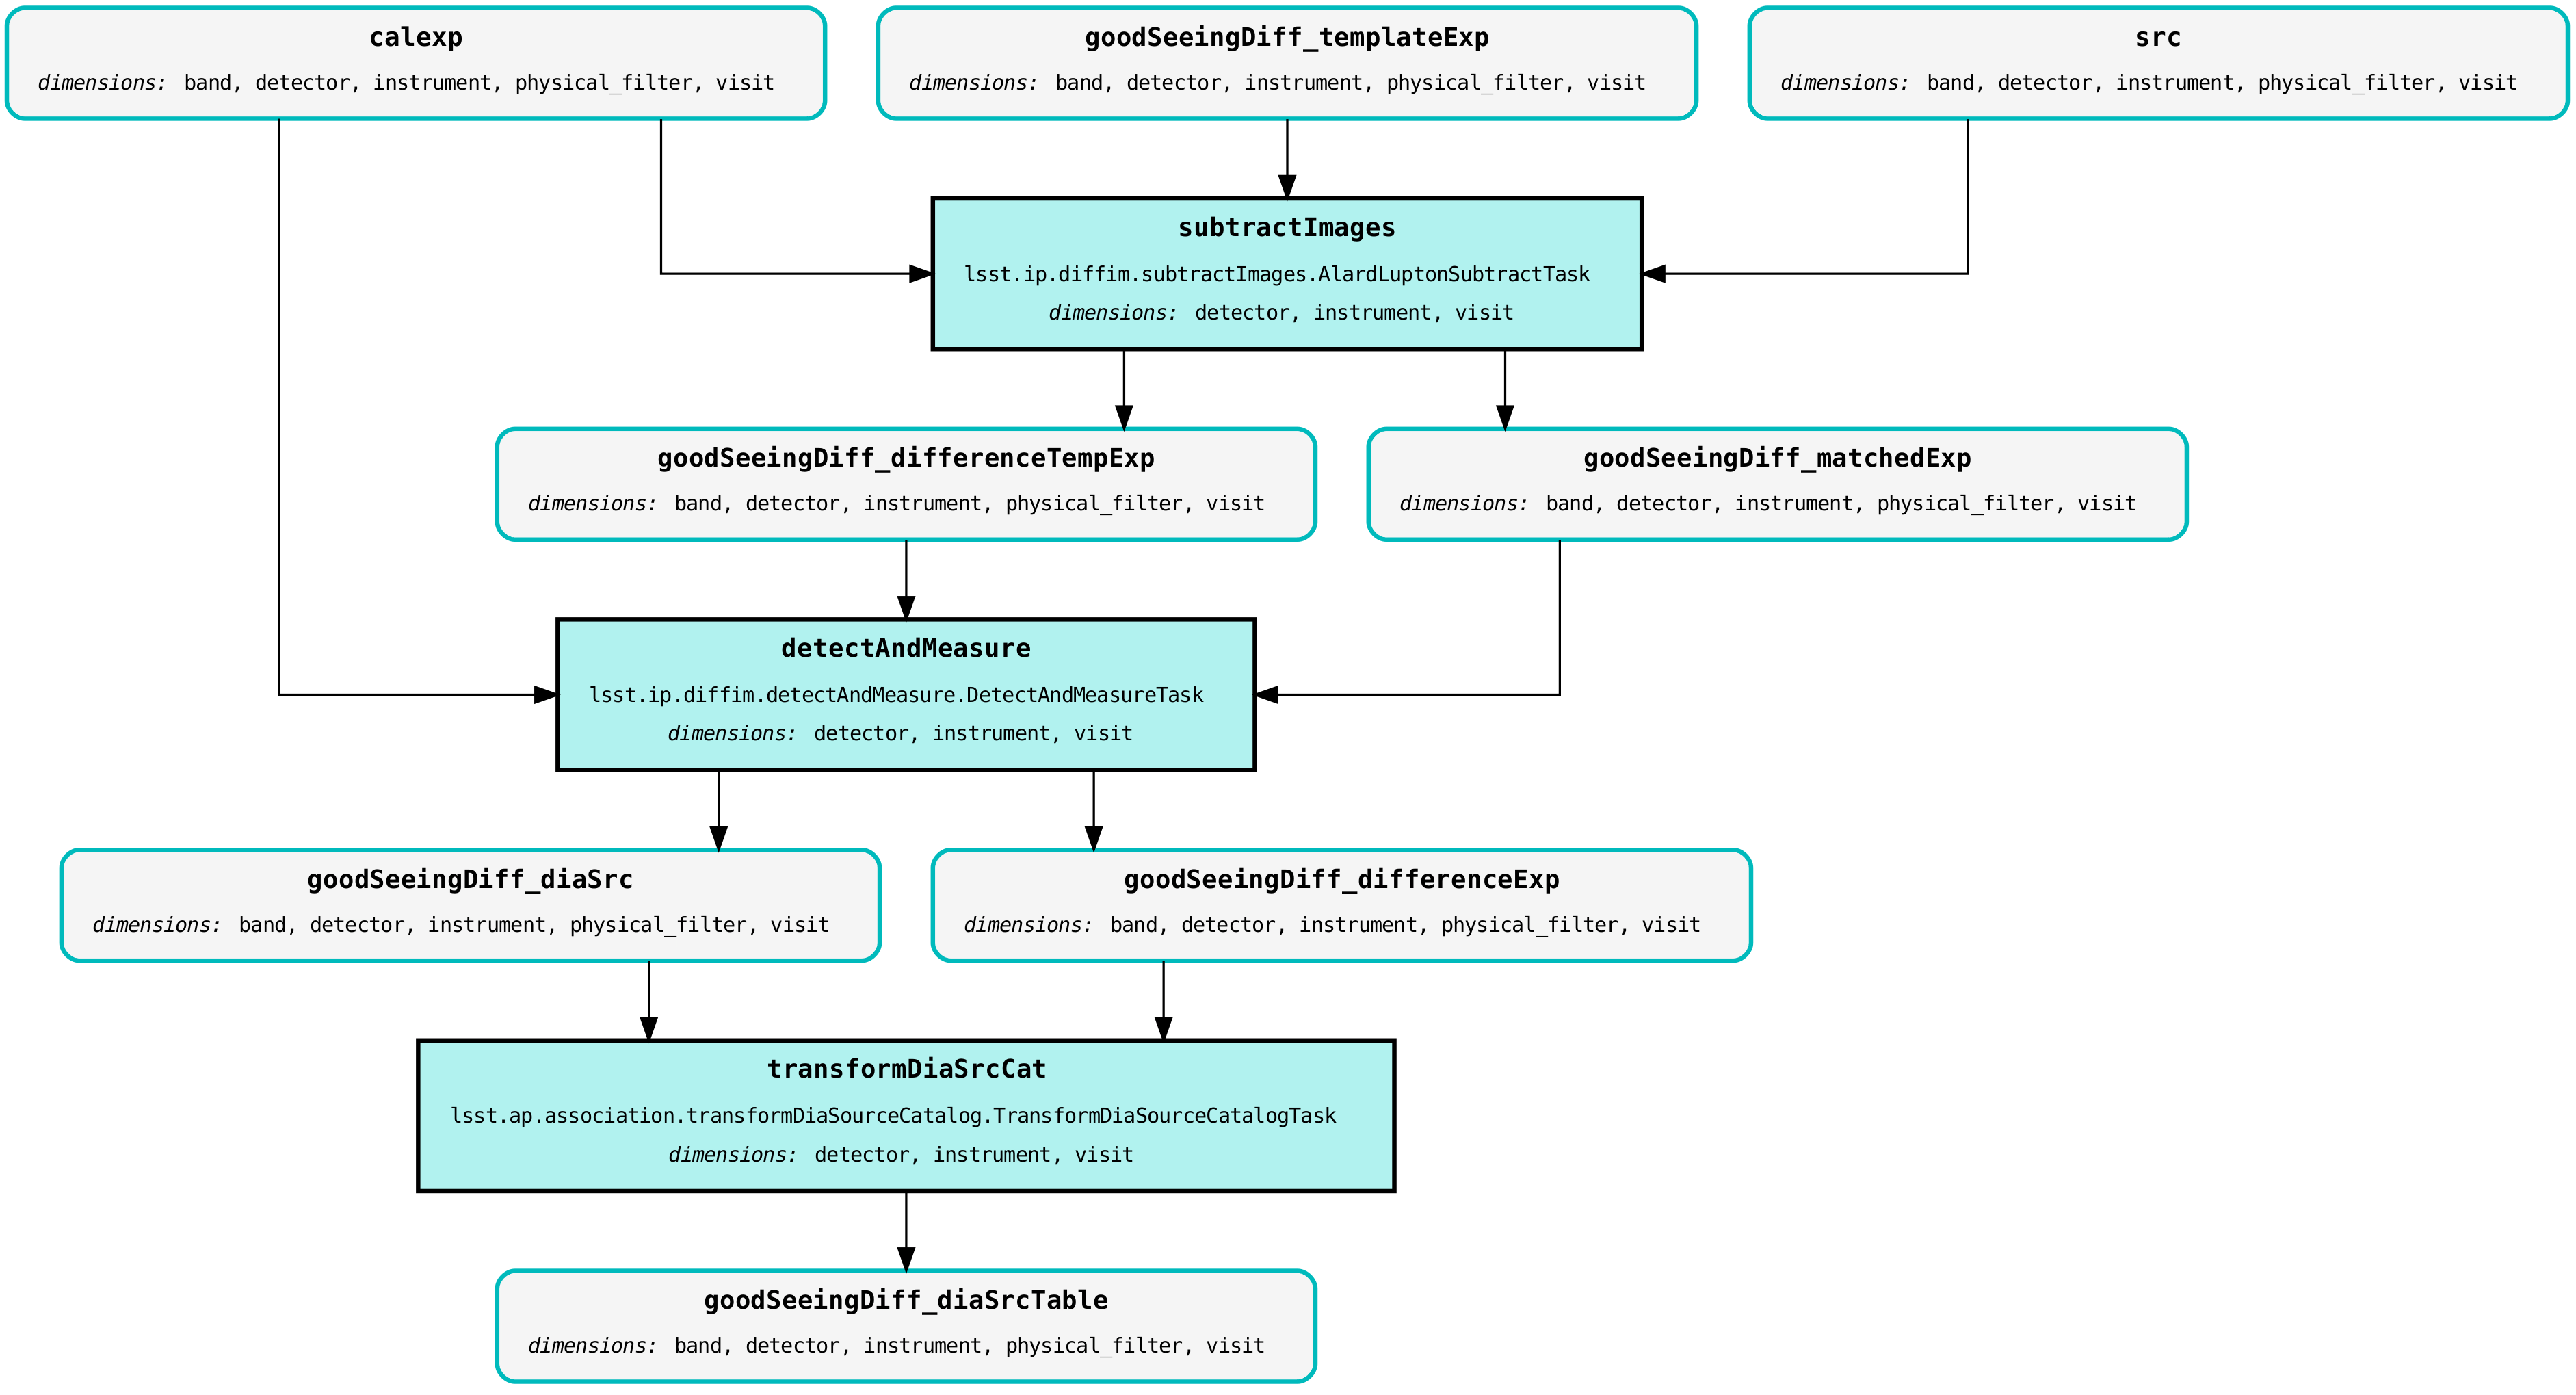
\includegraphics[width=0.9\textwidth]{pipeline.png}
  \caption{The lower part of the pipeline used for assessing the performance of the image differencing task. Note that the ``rbClassifier'' has been removed from the pipeline.}
  \label{fig:exposure_hist}
\end{figure}

The \texttt{transformDiaSrcCat} is kept in the pipeline, so the ``sky\_source'' are removed and do not clutter our data.
We used the \texttt{w\_2023\_38} version of the stack throughout the experiment.





\appendix
% Include all the relevant bib files.
% https://lsst-texmf.lsst.io/lsstdoc.html#bibliographies
\section{References} \label{sec:bib}
\renewcommand{\refname}{} % Suppress default Bibliography section
\bibliography{local,lsst,lsst-dm,refs_ads,refs,books}

% Make sure lsst-texmf/bin/generateAcronyms.py is in your path
\section{Acronyms} \label{sec:acronyms}
\addtocounter{table}{-1}
\begin{longtable}{p{0.145\textwidth}p{0.8\textwidth}}\hline
\textbf{Acronym} & \textbf{Description}  \\\hline

DM & Data Management \\\hline
\end{longtable}

% If you want glossary uncomment below -- comment out the two lines above
%\printglossaries





\end{document}
